\section{Preliminaries}
This section introduces the basic concepts needed to follow along with the rest of this thesis, while also putting some focus on notable historical work.
\subsection{Ray Tracing}
\label{path_tracing_basics}
\begin{figure}[H]
    \centering
    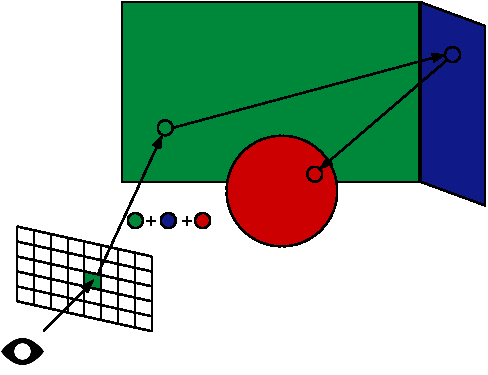
\includegraphics[width=250pt]{images/ray_tracing.pdf}
    \caption{Illustration of the path tracing process. A ray is cast into the scene for each pixel in the image plane. When an object is hit, its color is contributed to the pixel and a new ray is spawned.}
    \label{fig:path_trace}
\end{figure}
The basic technique of casting rays through each pixel in a viewing plane out into a three dimensional scene, was first proposed by Appel\cite{appel1968}. Whitted\cite{whitted_improved_1980} expanded on that approach by introducing a method that also captures reflections, shadows and refractions. This works by recursively spawning new rays when objects are hit, as described in figure \ref{fig:path_trace}. Each consecutive hit can contribute to a part of the pixels color. Whether and in what fashion secondary rays are created depends on the material of the encountered object. 

\begin{figure}[H]
    \centering
    \subcaptionbox{1 spp}{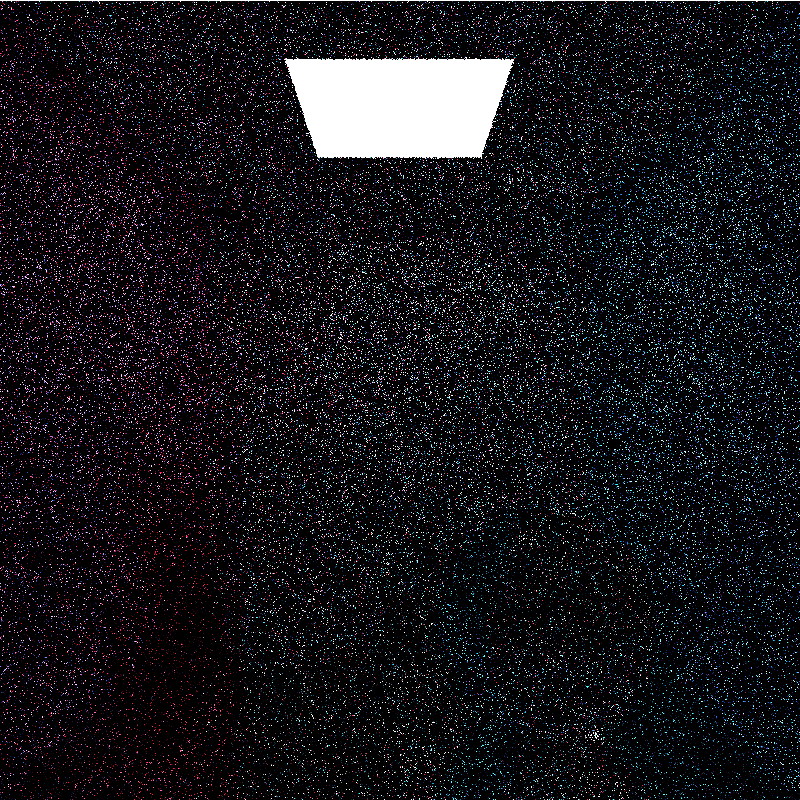
\includegraphics[width=0.2\textwidth]{images/cornell_1_spp.png}}
    \hfill
    \subcaptionbox{10 spp}{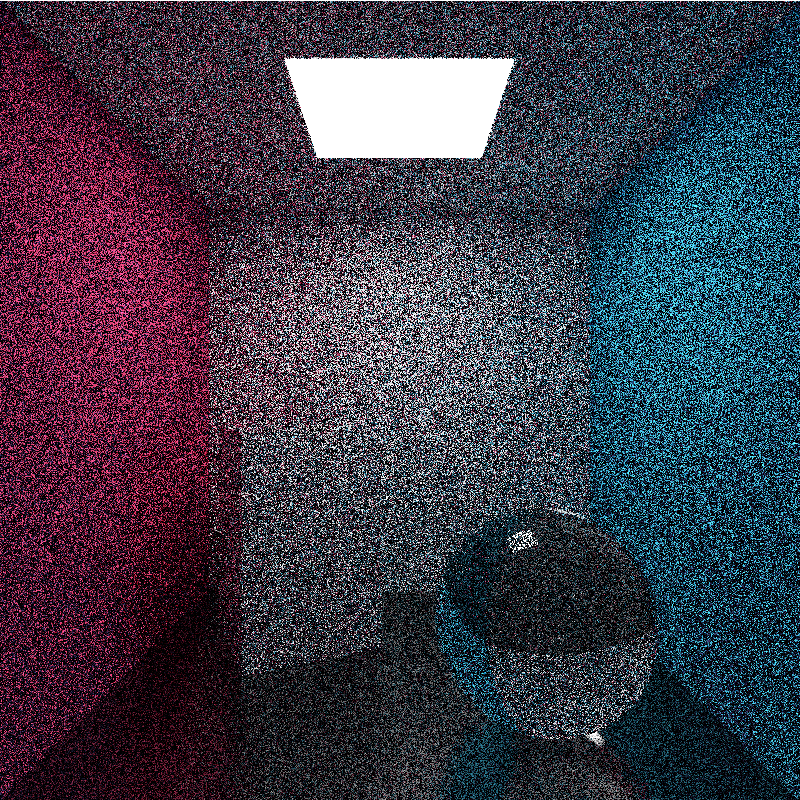
\includegraphics[width=0.2\textwidth]{images/cornell_10_spp.png}}
    \hfill
    \subcaptionbox{100 spp}{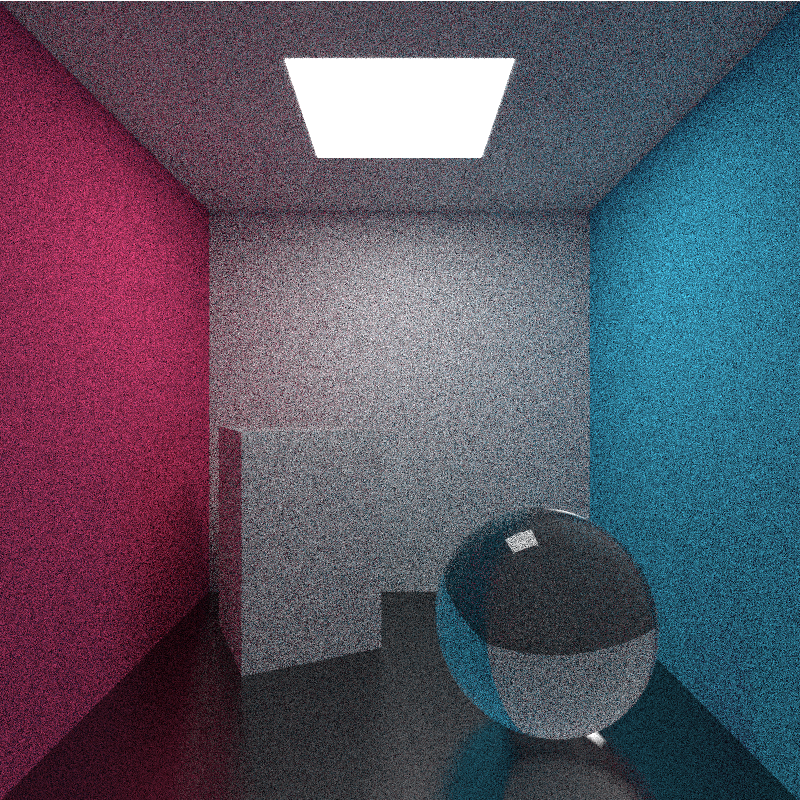
\includegraphics[width=0.2\textwidth]{images/cornell_100_spp.png}}
    \hfill
    \subcaptionbox{1000 spp}{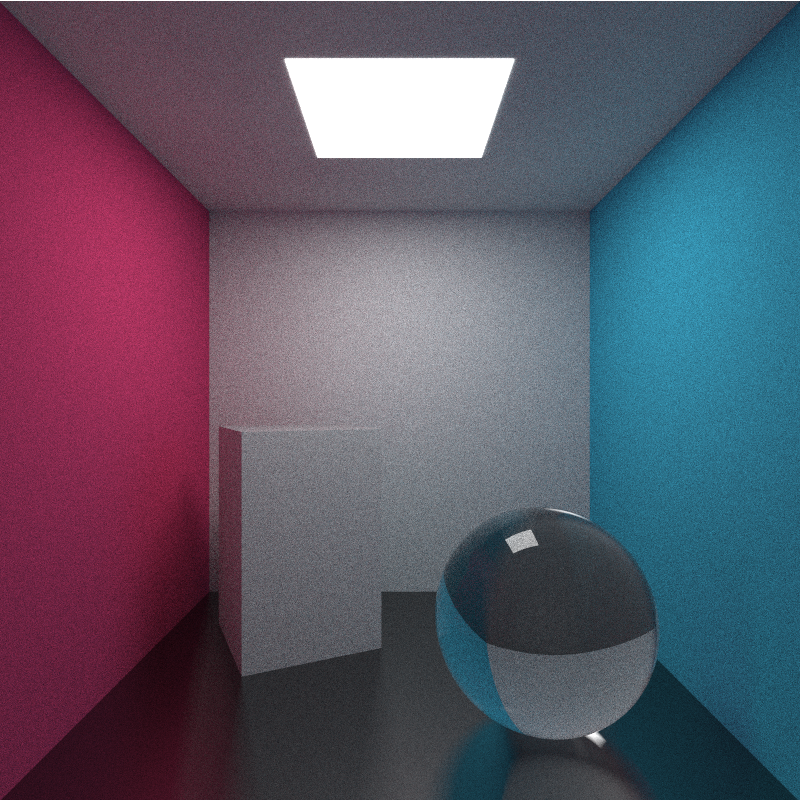
\includegraphics[width=0.2\textwidth]{images/cornell_1000_spp.png}}
    \caption{Noise at different sample-per-pixel (spp) values. Note that the images were rendered with implicit light sources. Noise is reduced using explicit light rays.}
    \label{fig:noise}
\end{figure}

The highest amount of realism can be achieved by a related concept called path tracing\cite{cook_distributed_1984, kajiya_rendering_1986}, which enables the accurate rendering of global illumination and distribution effects. Instead of casting a single ray per pixel, multiple samples are combined to more accurately simulate light transport through a scene. Each ray is cast with a slight offset within the pixel, which inherently solves the problem of aliasing. Secondary rays are scattered in random directions, depending on the surface they hit. Provided a sufficiently large sample size, this allows for a good approximation of the rendering equation\cite{kajiya_rendering_1986} and leads to very realistic results. Consequently, path tracing is very common in offline rendering, e.g., in film\cite{keller2015path_tracing_revolution} and visual effects, where relatively long render times can be tolerated. Given the limited time to process a frame in real-time, however, only allows to obtain a very limited number of samples. As seen in figure \ref{fig:noise}, 
these frames tend to suffer from high-frequency noise. Only through recent denoising techniques, further discussed in section \ref{denoising}, has this problem been overcome to make path tracing viable in real-time. A more detailed look at path tracing is presented in section \ref{path_tracer}.
\subsection{Acceleration Structures}
\label{acceleration_structure_basics}
\begin{figure}[H]
    \centering
    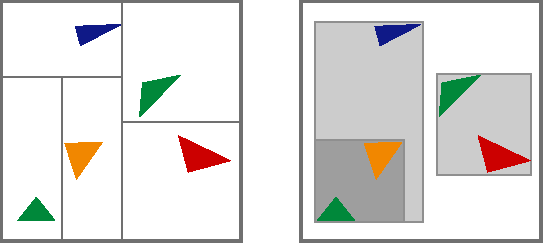
\includegraphics[width=250pt]{images/bvh_kd_tree.pdf}
    \caption{Example of space subdivision (left) and object subdivision (right).}
    \label{fig:subdiv}
\end{figure}
The essential and computationally most expensive step in path tracing is identifying the nearest intersection point for each ray. A naive approach would be to test the ray against all scene primitives, which in practice might be several million operations and thus too costly. Acceleration data structures are used to speed up that search process by arranging primitives in a spatial tree structure. Instead of checking all primitives, now the tree can be traversed to find the closest intersection. While doing so, all subtrees that are not hit by the ray can be neglected, reducing the number of total intersection tests drastically. Such data structures can be divided into two categories, space subdivision and object subdivision (figure \ref{fig:subdiv}). 

Space subdivision works by splitting the scene space recursively into smaller subregions, so each leaf in the resulting tree corresponds to a disjoint area in the full scene. This makes traversal of those structures very efficient, as the subregions can be tested in the order any ray passes through them. If a intersection is found, the traversal algorithm can be terminated without needing to check any further nodes. One of the limitations of such approaches is, that an object might lie in multiple subregions at once, i.e. multiple leaves might contain a pointer to the same object. This is problematic, because that way a point lying outside the associated region might be falsely identified as an intersection. The traversal algorithm as described would assume that point as the closest hit, even though there is no guarantee for that. Furthermore, this way the same object might be tested multiple times. Objects can be clipped to solve this problem, however, this introduces a certain computational cost. Alternatively, the traversal algorithm can be extended to also check whether or not a intersection point lies within a node's region. 

Object subdivision leads to trees with similar structure, however, each node is also associated with a bounding volume. Bounding volumes are a geometric shapes that enclose all primitives stored in any of the node's children. Axis-aligned bounding boxes (\acrshort{aabb}s) are the most popular volumes as they offer a good trade-off between intersection speed and tight fit around geometry. Bounding spheres offer the fastest intersection algorithm, but generally have larger volumes and oriented bounding boxes (\acrshort{obb}s) can provide the closest fit, but lack in intersection speed. When traversing such data structures, each child node needs to be checked as bounding volumes could overlap each other. A possible traversal algorithm is explained more detailed in section \ref{traversal}. In the rest of this section, basic \acrfull{bvh} construction algorithms are presented. 

A basic top-down algorithm starts at the root of the tree containing all scene primitives. The node is then split into two disjoint sets, which are set as children of the root. This process is repeated recursively for both children until some termination criteria is met and the given node is converted into a leaf. At each step, a bounding volume enclosing all primitives is assigned to the node. Given its exponential nature, splitting primitives into disjoint sets is a very complex problem. According to Popov et al.\cite{popov09harmful}, primitives can be split with a complexity of $O(n^6)$, which is not feasible in practice. As a result, primitives are generally split using axis-aligned planes. First, one splitting axis needs to be selected. Primitives are then ordered along that axis, most of the time according to their bounding volume centroid. Finding the split can then be done in three basic ways. A spatial median split cuts the bounding volume in half, object median uses a split with the same number of primitives in both halves and the most common approach splits primitives utilizing a cost model. 

The most common cost model is the \acrfull{sah}\cite{goldsmith_automatic_1987,macdonald_heuristics_1990}, which can be used to calculate the cost of a split as follows:
\[
    SAH(i)=S_L(i)p_L(i)+S_R(i)p_R(i)
\]
where $S_L(i)$ and $S_R(i)$ are the surface areas of the bounding boxes of the left and right subsets and $p_L(i)$ and $p_R(i)$ are the number of primitives in the subsets, respectively. Computing a full sweep SAH considering all primitives can be very expensive, thus a very popular method is binning SAH as proposed by Havran et al.\cite{havran06sahbin} and Wald et al.\cite{wald07fastConstruction}. In binning SAH primitives are projected into $b$ equally-spaced bins on which the SAH is then evaluated. 

Other cost functions include the occlusion heuristic\cite{vinkler12visibility} based on the assumed visibility of primitives and the ray distribution heuristic\cite{bittner09rdh}, which takes a sample the of the ray distribution into account. Both cost functions aim to improve the surface area heuristic, but might produce unstable results when used on their own, so it makes sense to combine those probabilities with the ones given by plain SAH.

Bottom-up construction\cite{Walter2008FastAC} starts by considering all primitives in clusters enclosed by bounding volumes. The two closest clusters are then merged to form a new node in the \acrshort{bvh} and the process is repeated until only one cluster is left, forming the trees root.
This approach is capable of producing trees with a better global cost compared to top-down approaches, which often only consider a local solution to cost functions. However, bottom-up construction in general is more expensive and the top levels might be poorly optimized due to the focus on lower levels.

Incremental construction\cite{goldsmith_automatic_1987} starts with an empty BVH and inserts primitives by traversing the tree and finding an appropriate leaf node. Once the number of primitives in a leaf gets too big, it is split into two new children. In general though, BVHs constructed this way are of lower quality making the approach less interesting. Nonetheless, it might still be useful if only parts of the input are available at the beginning, for example when streaming data.
\cleardoublepage